\subsection{单轨道解的三场分布}
本节对定理 \ref{thm:direct-HMB} 的单轨道三场解作数值计算. 图中使用规范变换前的场 $\widetilde q,\widetilde p,\eta$, 它们由 \eqref{eq:original-fields} 恢复. 取参数
\begin{equation}\label{eq:numerical-parameters}
q_0=1,\qquad a=2,\qquad\eta_0=0.6,\qquad
\alpha=1,\qquad\beta=0.1,\qquad b=1.5,
\end{equation}
范数常数由式 \eqref{eq:onec} 给定, 场值由四维留数系统及无穷远、共振点的重构公式计算. 图 \ref{fig:one} 展示光场的局域振荡及同一区域内的极化和粒子数反转.
\begin{figure}[!htbp]
\centering
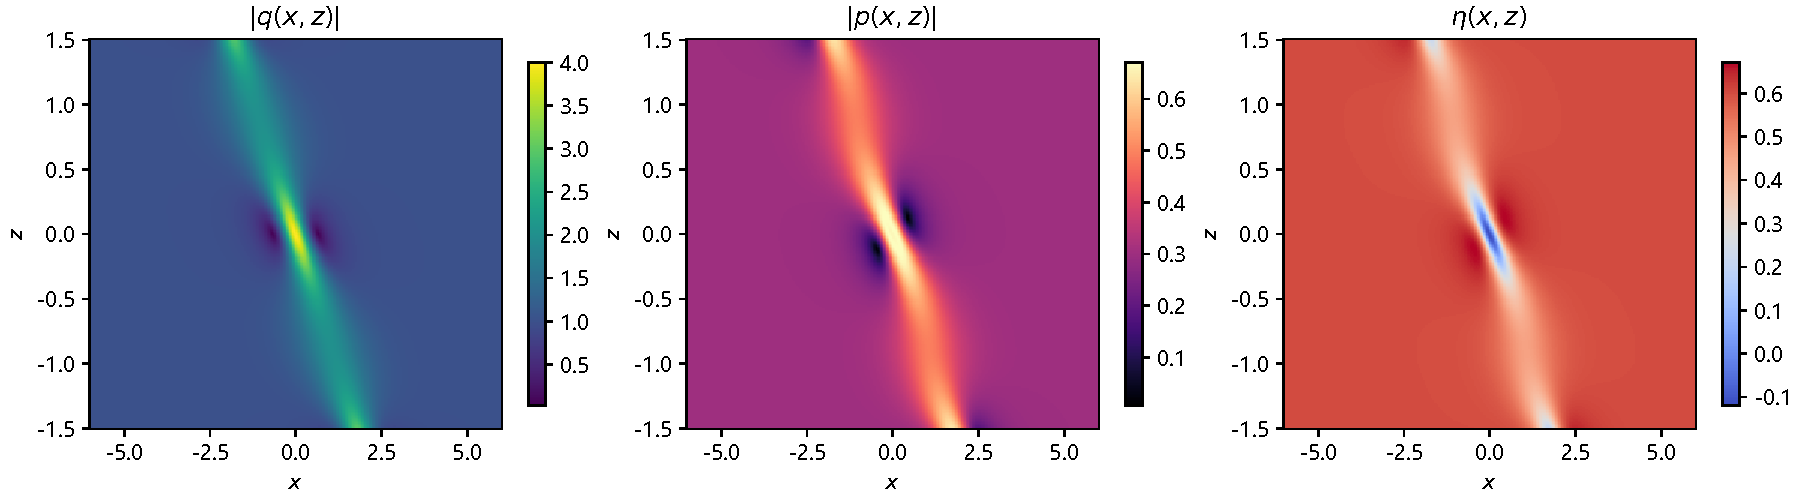
\includegraphics[width=\textwidth]{figures/one-soliton-fields.pdf}
\caption{单轨道物理三场 $|\widetilde q|,|\widetilde p|,\eta$ 的曲面 (上排) 与等值图 (下排). 参数见 \eqref{eq:numerical-parameters}; $x\in\lbrack-6,6\rbrack$, $t\in\lbrack-1.5,1.5\rbrack$.}
\label{fig:one}
\end{figure}

\FloatBarrier
\subsection{传播速度与内部振荡}
将背景传播因子分解为
\begin{align}
A_b=\operatorname{Re}F(\ii b)
&=-4\beta b^2-2\beta q_0^2-\dfrac{\eta_0}{a^2+b^2},\label{eq:velocity}\\
B_b=\operatorname{Im}F(\ii b)
&=-\alpha b-\dfrac{\eta_0b}{a(a^2+b^2)}.\label{eq:frequency}
\end{align}
于是 $s=\kappa X-\ii\kappa B_bt$, 其中 $X=x-A_bt$. 显式矩阵 $P$ 关于 $x,t$ 的依赖由
\[
T=e^{2s}=e^{2\kappa X}e^{-2\ii\kappa B_bt}
\]
确定. 固定 $X$ 时, 若 $B_b\ne0$, 去相位三场具有周期
\begin{equation}\label{eq:internal-period}
T_t=\dfrac{\pi}{\kappa|B_b|}.
\end{equation}
若 $\alpha=-\dfrac{\eta_0}{a(a^2+b^2)}$, 则 $B_b=0$, 去相位三场仅依赖 $X$. 原场的模 $|\widetilde q|,|\widetilde p|$ 和反转 $\eta$ 也具有周期 \eqref{eq:internal-period}; 复场 $\widetilde q,\widetilde p$ 具有同一随动周期当且仅当 $\Omega T_t\in2\pi\mathbb Z$.

由 $P^2=P=P^\dagger$ 和 $\tr P=1$, 有 $|P_{12}|^2=P_{11}(1-P_{11})\le\dfrac{1}{4}$. 因而
\begin{equation}\label{eq:amplitude-bound}
|\widetilde q(x,t)|\le q_0+2b,\qquad |\widetilde q(0,0)|=q_0+2b.
\end{equation}
后一等式使用 $T(0,0)=1$ 和 $P_{12}(0,0)=\dfrac{1}{2}$. $P$ 在 $X\to\pm\infty$ 时趋于端态投影, 修正项为 $O(e^{-2\kappa|X|})$, 所以局域化尺度由 $\kappa$ 决定.

参数 \eqref{eq:numerical-parameters} 给出 $A_b=-1.196$、$B_b=-1.572$ 和 $T_t\approx1.78748466439$. 图 \ref{fig:dynamics} 左图比较 $t=0,\dfrac{T_t}{4},\dfrac{T_t}{2}$ 时的随动截面; 右图比较 $\alpha=-0.048,0.5,1$ 时的中心光场模. 后两者的周期分别约为 $3.41840132897$ 和 $1.78748466439$, 而 $\alpha=-0.048$ 对应行波.
\begin{figure}[htbp]
\centering
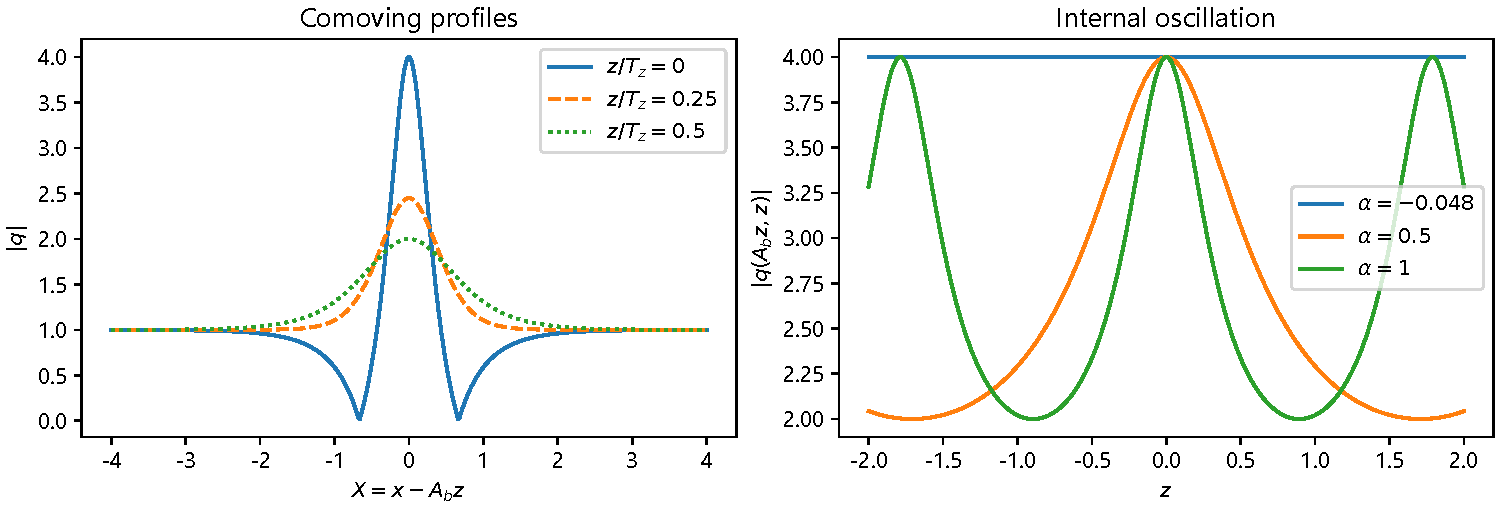
\includegraphics[width=\textwidth]{figures/one-soliton-dynamics.pdf}
\caption{单轨道光场的局域化与内部振荡. (a) 参数 \eqref{eq:numerical-parameters} 下的随动截面. (b) 改变 $\alpha$ 时 $|\widetilde q(A_bt,t)|$ 的变化, 其余参数固定.}
\label{fig:dynamics}
\end{figure}

\FloatBarrier
\subsection{参数影响与数值验证}
$\beta$ 改变式 \eqref{eq:velocity} 中的传播速度, 而不改变式 \eqref{eq:frequency} 中的内部频率. 图 \ref{fig:velocity} 取 $\beta=0,0.15$, 相应的 $A_b$ 为 $-0.096,-1.746$; 两者均有 $B_b=-1.572$ 和相同的随动周期. 虚线 $x=A_bt$ 表示中心轨迹.
\begin{figure}[htbp]
\centering
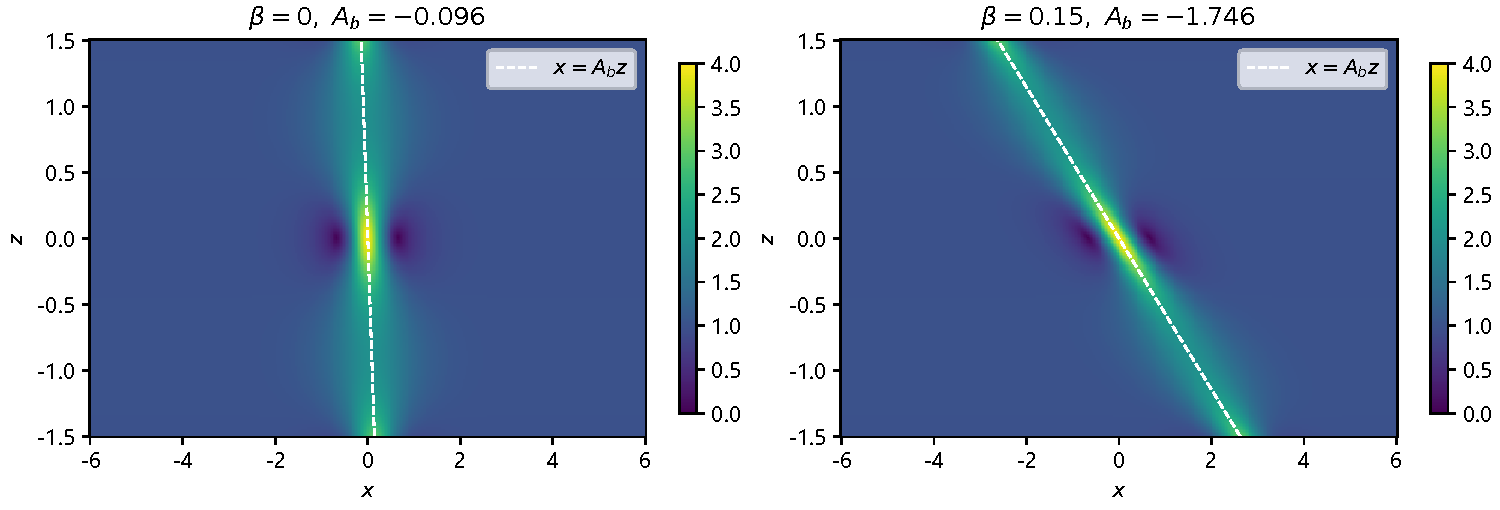
\includegraphics[width=\textwidth]{figures/one-soliton-velocity.pdf}
\caption{改变 $\beta$ 时的光场传播速度. 两图分别取 $\beta=0,0.15$, 其余参数同 \eqref{eq:numerical-parameters}; 白色虚线为 $x=A_bt$.}
\label{fig:velocity}
\end{figure}

对参数 \eqref{eq:numerical-parameters}, 采用 70 位十进制精度求解留数系统并对重构场求导, 得到表 \ref{tab:direct-residuals}. 导数由重构表达式直接计算. 双精度绘图实现与高精度实现的三个场在相同样点上的差均小于 $10^{-14}$; 等值图网格上的 Bloch 长度平方偏差及 $\eta$ 虚部均小于 $10^{-14}$. 两端 $x=\pm30$ 的三场误差均小于 $5.02\times10^{-29}$.
\begin{table}[htbp]
\centering
\caption{单轨道三场的高精度核验, 表内为样点最大绝对残差的向上舍入值}
\label{tab:direct-residuals}
\begin{tabular}{lc}
\toprule 检验对象 & 最大绝对误差\\\midrule
光场方程 & $1.87\times10^{-69}$\\
极化方程 & $8.26\times10^{-71}$\\
粒子数反转方程 & $1.50\times10^{-70}$\\
空间 Lax 方程 & $4.82\times10^{-70}$\\
时间 Lax 方程 & $1.95\times10^{-69}$\\
两共振原像的介质重构 & $1.12\times10^{-71}$\\
Bloch 长度平方 & $4.77\times10^{-72}$\\
\bottomrule
\end{tabular}
\end{table}


\subsection{数值计算的方法与结论范围}
数值图像由已证明的单轨道重构公式求值得到.
计算同时采用有限维留数系统与投影表达式, 用两种实现的相互比较核对代数重构.
三场方程、Lax 方程、Bloch 约束和两共振原像一致性的残差分别检验,
空间端态则在较大正负 $x$ 处核对.
这些样点检验与第 \ref{ch:verification} 节的解析证明相互配合:
解析证明建立全部实 $x,t$ 上的方程与边界, 数值结果展示局域结构及参数作用.

本文由此完成非零背景的直接散射、共振相容性、条件性 RHP 重构和指定单轨道的全局验证.
一般含反射数据的 RHP 可解性, 以及一般多轨道留数矩阵的全局非退化性,
需要进一步的分析, 不由本文的有限样点计算推出.
